\documentclass[hyperref=unicode]{beamer}

\usepackage[absolute,overlay]{textpos}
\usepackage{graphicx}
\usepackage{adjustbox}
\usepackage{chemfig}
\usepackage[version=4]{mhchem}
\usepackage{wrapfig}
\usepackage{multirow}
\adjustboxset*{center}
\usepackage{caption}
\usepackage{chemformula}
\usepackage{elements}

%dělení slov
\usepackage{ragged2e}
\let\raggedright=\RaggedRight
%konec dělení slov

\usepackage{fontspec}
\usepackage{unicode-math}

\usepackage{polyglossia}
\setdefaultlanguage{czech}

\def\uv#1{„#1“}

\mode<presentation>{\usetheme{Madrid}}
\DefineNamedColor{named}{pozadi}{RGB}{200,200,200}
\usecolortheme{crane}

\setbeamertemplate{footline}[frame number]

\addtobeamertemplate{frametitle}{
	\let\insertframetitle\insertsectionhead}{}
\addtobeamertemplate{frametitle}{
	\let\insertframesubtitle\insertsubsectionhead}{}

\makeatletter
\CheckCommand*\beamer@checkframetitle{\@ifnextchar\bgroup\beamer@inlineframetitle{}}
\renewcommand*\beamer@checkframetitle{\global\let\beamer@frametitle\relax\@ifnextchar\bgroup\beamer@inlineframetitle{}}
\makeatother
\setbeamercolor{section in toc}{fg=blue}
\setbeamertemplate{section in toc shaded}[default][100]

\title[Crisis]
{Roztoky, pH}

\subtitle{Aktivita, iontová síla, kyseliny a zásady, pH}

\titlegraphic{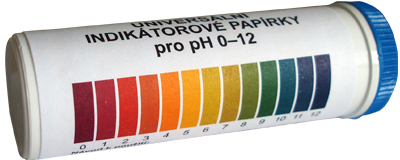
\includegraphics[keepaspectratio,width=7cm]{img/ph.jpg}}
\date{}

\begin{document}
\frame{\titlepage}

\section{Aktivita roztoku}
\frame{
	\frametitle{}
	\vfill
	\textbf{Aktivita roztoku}
	\begin{itemize}
	\item Popisuje reálné chování roztoku. Na rozdíl od ideálního roztoku, se v reálném roztoku částice navzájem ovlivňují.
	\item Aktivita jakékoliv čisté látky v kondenzovaném stavu (kapalina nebo pevná látka) je jednotková.
	\item Aktivita plynu závisí na jeho parciálním tlaku, obvykle se označuje jako \textbf{fugacita}.
	\item $\mu_i = \mu_i^0 + \textrm{RT} \ln a_i$
	\item $\mu_i$ - chemický potenciál, $\mu_i^0$ - standardní chemický potenciál
	\item Ativitu lze vyjádřit jako součin molární koncentrace a aktivitního koeficientu
	\item a $ = \gamma $c
	\item Aktivitní koeficient je úměrný náboji iontů v roztoku a iontové síle roztoku
	\end{itemize}
	\vfill
}

\subsection{Iontová síla roztoku}
\frame{
	\frametitle{}
	\vfill
	\textbf{Iontová síla roztoku}
	\begin{itemize}
	\item $\log \gamma = -0,509\textrm{z}^2\sqrt{\textrm{I}}$
	\item I - iontová síla roztoku - popisuje množství iontů v roztoku
	\item $I = \frac{1}{2}\sum\limits_{i=0}^n \textrm{c}_i \textrm{z}^2_i$
	\item c$_i$ -- molalita; z$_i$ -- náboj; 0,509 -- konstanta pro vodné roztoky při 25~$^\circ$C
	\end{itemize}
	\vfill
}

\subsection{Střední aktivitní koeficienty ve vodných roztocích při 25 $^\circ$C}
\frame{
	\frametitle{}
	\vfill
	\textbf{Střední aktivitní koeficienty ve vodných roztocích při 25 $^\circ$C}
	\begin{tabular}{|l||r@{,}l|r@{,}l|r@{,}l|r@{,}l|}
	\hline
	$c_m [mol.kg^{-1}]$ & 0 & 1 & 1 & 0 & 4 & 0 & 10 & 0 \\\hline
	HCl & 0 & 796 & 0 & 809 & 1 & 762 & 10 & 44 \\\hline
	NaOH & 0 & 766 & 0 & 678 & 0 & 903 & 3 & 52 \\\hline
	KOH & 0 & 798 & 0 & 756 & 1 & 352 & 6 & 22 \\\hline
	\ce{H_2SO_4} & 0 & 265 & 0 & 130 & 0 & 171 & 0 & 553 \\\hline
	\ce{AgNO_3} & 0 & 734 & 0 & 429 & 0 & 210 & \multicolumn{2}{|c|}{} \\\hline
	\ce{Ca(NO_3)_2} & 0 & 48 & 0 & 35 & 0 & 42 & \multicolumn{2}{|c|}{} \\\hline
	\end{tabular}
	\vfill
	\footnotesize VOHLÍDAL, Jiří. Chemické tabulky. Praha: SNTL, 1982.
}

\section{Kyseliny a zásady}
\frame{
	\frametitle{}
	\vfill
	\textbf{Kyseliny a zásady}
	\begin{itemize}
	\item Arrheniova teorie - kyseliny jsou látky, které ve vodném roztoku uvolňují ion \ce{H^+}, resp. \ce{H_3O^+}, zásady uvolňují \ce{OH^-}
	\item Br\o nstedova teorie - kyseliny jsou donory protonů, zásady jejich akceptory
	\item Lewisova teorie - kyseliny jsou akceptorem elektronových párů, zásady donorem
	\begin{itemize}
		\item \ce{$\underset{\text{zásada}}{\ce{|NH3}}$ + $\underset{\text{kyselina}}{\ce{BF3}}$ -> NH3\bond{->}BF3}
	\end{itemize}
	\end{itemize}
	\vfill
}

\frame{
	\frametitle{}
	\vfill
	\begin{itemize}
	\item Silné kyseliny a zásady - zcela disociují
	\item \ce{HCl + H2O -> H3O^+ + Cl^-}
	\item \ce{NaOH -> Na^+ + OH^-}
	\item Slabé kyseliny a zásady - disociují pouze z části
	\item \ce{CH3COOH + H2O <=>[\text{$\textrm{pK}_a$}] H3O^+ + CH3COO^-}
	\item \ce{NH3 + H2O <=>[\text{$\textrm{pK}_b$}] OH^- +N{\text{H}$_4^+$}}
	\item $\textrm{pK}_a$, $\textrm{pK}_b$ - disociační konstanta
	\item \scalebox{1.2}{$\textrm{K}_a = \frac{\ce{[H3O^+][Cl^-]}}{\ce{[HCl]}}$}; \scalebox{1.2}{$\textrm{K}_b = \frac{\ce{[OH^-][N{\textrm{H}_4^+}]}}{\ce{[NH3]}}$}
	\item $\textrm{pK}_a = -\log \textrm{K}_a; \textrm{pK}_b = -\log \textrm{K}_b$
	\end{itemize}
	\vfill
}

\frame{
	\frametitle{}
	\vfill
	\begin{columns}[T]
		\begin{column}{.5\textwidth}
			\begin{tabular}{|l|lr@{,}l|}
				\hline
				Kyselina & \multicolumn{3}{|c|}{pK$_a$} \\\hline
				Fenol & & 9 & 89 \\\hline
				\ce{H2CO3} & pK$_{a1}$ & 6 & 35 \\\hline
				& pK$_{a2}$ & 10 & 33 \\\hline
				\hline
				kys. octová & & 4 & 75 \\\hline
				\ce{HNO2} & & 3 & 29 \\\hline
				HF & & 3 & 2 \\\hline
				\ce{H3PO4} & pK$_{a1}$ & 2 & 16 \\\hline
				& pK$_{a2}$ & 7 & 21 \\\hline
				& pK$_{a3}$ & 12 & 32 \\\hline
				\hline
				\ce{H3PO3} & pK$_{a1}$ & 2 & 00 \\\hline
				& pK$_{a2}$ & 6 & 58 \\\hline
				\hline
				kys. trichloroctová & & 0 & 70 \\\hline
			\end{tabular}
		\end{column}
	
		\begin{column}{.5\textwidth}
			\begin{tabular}{|l|lr@{,}l|}
				\hline
				Zásada & \multicolumn{3}{|c|}{pK$_b$} \\\hline
				\ce{Be(OH)2} & & 10 & 30 \\\hline
				nikotin & pK$_{b1}$ & 5 & 98 \\\hline
				& pK$_{b2}$ & 10 & 88 \\\hline
				\hline
				\ce{NH3} & & 4 & 75 \\\hline
				\ce{AgOH} & & 3 & 96 \\\hline
			\end{tabular}
		\end{column}
	\end{columns}
	\vfill
}

\frame{
	\frametitle{}
	\vfill
	\textbf{Konjugované páry kyselina a zásad}
	\begin{itemize}
	\item Liší se o \ce{H^+}
	\item \ce{HCl + H2O -> H3O^+ + Cl^-}
	\item \ce{HCl -> Cl^-}
	\item \ce{H2O -> H3O^+}
	\item Konjugovaná zásada k silné kyselině je slabá
	\item Konjugovaná kyselina k slabé zásadě je silná
	\end{itemize}
	\vfill
}

\frame{
	\frametitle{}
	\vfill
	\textbf{Autoionizace vody}
	\begin{itemize}
		\item Voda je amfoterní, chová se jako kyselina i zásada
		\item \ce{2 H2O <-> H3O^+ + OH^-}
		\item Iontový součin vody: 
		\begin{itemize}
			\item $\textrm{K}_w = \ce{[H^+][OH^-]} = 1.10^{-14}\ \textrm{mol.dm}^{-3}$
		\end{itemize}
		\item $\textrm{pK}_w = -\log \textrm{K}_w = 14$
		\item Pro konjugovaný pár kyselina-zásada platí: 
		\begin{itemize}
			\item $\textrm{K}_a\textrm{K}_b = \textrm{K}_w$
			\item $\textrm{pK}_a + \textrm{pK}_b = \textrm{pK}_w$
		\end{itemize}
	\end{itemize}
	\vfill
}

\subsection{pH a pOH}
\frame{
	\frametitle{}
	\vfill
	\begin{itemize}
	\item $\textrm{pH} = -\log\ \textrm{a}_{H_3O^+} = -\log[\ce{H3O^+}]$
	\item $\textrm{pOH} = -\log\ \textrm{a}_{OH^-} = -\log[\ce{OH^-}]$
	\item pH + pOH = 14,00
	\item pH $<$ 7 - roztok je kyselý
	\item pH = 7 - roztok je neutrální
	\item pH $>$ 7 - roztok je zásaditý
	\end{itemize}
	\begin{center}
	\begin{tabular}{|c|c|c|c|}
	\hline
	pH & pOH & [\ce{H^+}] & [\ce{OH^-}] \\\hline
	0 & 14 & 1,0 & 10$^{-14}$ \\\hline
	2 & 12 & 0,01 & 10$^{-12}$ \\\hline
	4 & 10 & 0,0001 & 10$^{-10}$ \\\hline
	6 & 8 & 10$^{-6}$ & 10$^{-8}$ \\\hline
	8 & 6 &10$^{-8}$ & 10$^{-6}$ \\\hline
	10 & 4 & 10$^{-10}$ & 0,0001 \\\hline
	12 & 2 & 10$^{-12}$ & 0,01 \\\hline
	14 & 0 & 10$^{-14}$ & 1,0 \\\hline
	\end{tabular}
	\end{center}
	\vfill
}

\subsection{Výpočet pH}
\frame{
	\frametitle{}
	\vfill
	\textbf{Silné kyseliny a zásady}
	\begin{itemize}
	\item $\textrm{pH} = -\log[\ce{H^+}] = -\log\ c_{kys} = 14 + \log\ c_{zas} $
	\item pH = 14 - pOH
	\end{itemize}
	\textbf{Slabé kyseliny a zásady}
	\begin{itemize}
	\item $[\ce{H^+}] = \sqrt{K_a[HA]_0}$
	\item $\textrm{pH} = \frac{1}{2}\textrm{pK}_a - \frac{1}{2}\log c_{kys}$
	\item $\textrm{pH} = 14 - \frac{1}{2}\textrm{pK}_b + \frac{1}{2}\log c_{zas}$
	\end{itemize}
	\textbf{Soli silné kyseliny i zásady}
	\begin{itemize}
	\item \ce{NaCl + H2O -> Na^+ + Cl^- + H2O}
	\item \ce{KNO3 + H2O -> K^+ + NO3^- + H2O}
	\item Nedochází k ovlivnění [\ce{H^+}] ani [\ce{OH^-}]
	\end{itemize}
	\vfill
}

\subsection{Roztoky solí}
\frame{
	\frametitle{}
	\vfill
	\textbf{Soli slabé kyseliny nebo slabé zásady}
	\begin{itemize}
	\item \ce{NH4NO3 + H2O -> NH4^+ + NO3^- + NH3 + H^+}
	\item $\textrm{pH} = 7 - \frac{1}{2}(\textrm{pK}_b + \log c)$ \\
	\rule{6cm}{0.4pt}
	\item \ce{NaF + H2O -> Na^+ + F^- + HF + OH^-}
	\item $\textrm{pH} = 7 + \frac{1}{2}(\textrm{pK}_a + \log c)$ \\
	\rule{6cm}{0.4pt}
	\item \ce{NH4F + H2O -> NH4^+ + F^- + NH3 + H^+ + HF + OH^-}
	\item $\textrm{pH} = 7 + \frac{1}{2}(\textrm{pK}_a - \textrm{pK}_b)$
	\end{itemize}

	\textbf{Příklad}
	\begin{itemize}
	\item $\textrm{pK}_a (\ce{HF}) = 3,17$
	\item $\textrm{pK}_b (\ce{NH3}) = 4,75$
	\item $\textrm{pH} = 7 + \frac{1}{2}(3,17 - 4,75) = 6,21$
	\end{itemize}
	\vfill
}

\subsection{Pufry, tlumivé (ústojné) roztoky}
\frame{
	\frametitle{}
	\vfill
	\begin{itemize}
	\item Jde o směs slabé kyseliny a její soli nebo slabé zásady a její soli
	\item Příkladem je např. acetátový pufr - směs kyseliny octové a octanu sodného
	\item Rovnováhy v pufru lze popsat rovnicemi
	\item \ce{CH3COOH + H2O <-> CH3COO^- + H3O^+}
	\item \ce{CH3COONa + H2O <-> CH3COOH + Na^+ + OH^-}
	\item Přídavkem kyseliny vzniknou molekuly kyseliny octové, přídavkem zásady ionty octanu. pH roztoku se nezmění.
	\item $\textrm{pH} = \textrm{pK}_a + \log \frac{[A^-]}{[HA]}$
	\item $\textrm{pH} = 14 - \textrm{pK}_b + \log \frac{[B]}{[BH^+]}$
	\end{itemize}
	\begin{center}
	\begin{tabular}{|c|c|c|}
	\hline
	Pufr & Složení & Rozsah pH \\\hline
	Acetátový & \ce{CH3COOH}/\ce{CH3COONa} & 3,8 - 5,8 \\\hline
	Fosfátový & \ce{NaH2PO4}/\ce{Na2HPO4} & 6,2 - 8,2 \\\hline
	Borátový & \ce{H3BO3}/\ce{Na2B4O7} & 8,25 - 10,25 \\\hline
	\end{tabular}
	\end{center}
	\vfill
}

\subsection{Příklad výpočtu pH slabé kyselina}
\frame{
	\frametitle{}
	\vfill
	\emph{Jaké je pH 0,2 M kyseliny octové, p$K_a$ = 4,76?}
	\hrule \hrule


	\ce{CH3COOH <-> CH3COO^- + H^+}

	$K_a = 10^{-\textrm{pK}_a} = 10^{-4.76} = 0,000017$

	$K_a = \frac{[\ce{CH3COO^-}][\ce{H^+}]}{[\ce{CH3COOH}]} = \frac{x.x}{0,2-x}$

	Dosadíme za $K_a$ a upravíme získaný výraz, čímž dostaneme kvadratickou rovnici:

	$x^2 + 0,000017x - 0,0000034 = 0$

	Kvadratickou rovnici vyřešíme pomocí diskriminantu:

	$x_{1,2} = \frac{-b \pm \sqrt{D}}{2a} = \frac{-b \pm \sqrt{b^2 - 4ac}}{2a} = \frac{-0,000017 \pm \sqrt{0,000017^2 - 4.1.(-0,0000034)}}{2.1}$

	Ze dvou vypočítaných kořenů zvolíme ten kladný, koncentrace totiž nemůže být záporná.

	$x = 0,0018$

	$\textrm{pH} = -\log[H^+] = -\log0,018 = 2,74$
	\vfill
}
\iffalse
\section{Další informace}
\frame{
	\frametitle{}

	\href{http://z-moravec.net/chemie/zaklady-chemie/}{http://z-moravec.net/}
}
\fi

\end{document}